%
%===============>>  ГРУППА 10-2 МОДУЛЬ 8  <<=============
%
\setmodule{8}

%BEGIN_FOLD % ====>>_____ Занятие 1 _____<<====
\begin{class}[number=1]
	\begin{listofex}
		\item Решите уравнения: %c109 21 24 25 a
		\begin{tasks}
			\task \((x^2-9)\lg(-x)=0  \)
			\task \( \log_2(x^2-7)=\log_{4-x}(4-x) \)
			\task \( \log_{11}(y^2-35)=\log_{7-y}1 \)
			%\task \( \dfrac{ \log_{x+1}^2 (x-1) + \log_5^2(2x-5) }{ \log_{x+1}^2 (x-1) + \log_5^2(x-2) }=1 \) НА ОЧЕНЬ ПОТОМ
			\task \( \log_2^2x-\log_2x^{-7}+12=0 \)
		\end{tasks}
		\item Решите системы неравенств: %диагн 2 с301 v2 10-11
		\begin{tasks}(2)
			\task \( \begin{cases} \log_{0,2}(2x-7) \le -2 \\ \log_3 (x-5) \le 3 \end{cases} \)
			\task \( \begin{cases} \log_3 (25-x^2) \ge 2 \\ \log_5 (x^2+9) \ge 2 \end{cases} \)
		\end{tasks}
		\item Решите неравенства: %c321 a 7 8 9 10
		\begin{tasks}
			\task \( \log_3(x+2)+\log_3(8-x)\le 1 + \log_3(x+4) \)
			\task \( \log_7(4x+11)-\log_7(25-x^2)\ge \sin \left( \dfrac{ 11\pi }{ 2 } \right) \)
			\task \( \log_3(x+5) \ge \log_{9-x}(9-x) \)
			\task \( 1-\dfrac{ 1 }{ \log_{x-4}0,2 } \le \dfrac{ 2 }{ \log_{x+20}25 } \)
		\end{tasks}
		
	\end{listofex}
\end{class}
%END_FOLD

%BEGIN_FOLD % ====>>_____ Занятие 2 _____<<====
\begin{class}[number=2]
	\begin{listofex}
		\item Решите уравнения: %109 б 8 10 11 15 17 trening10
		\begin{tasks}(2)
			\task \( \log_2^2 x - \log_2 x^{-7} + 12 = 0 \)
			\task \( \log_{y^2}17=\log_{4+3y}17 \)
			\task \( \dfrac{ (x-9)(x-7) }{ \log_3(x+8) }=0 \)
			%\task \( \dfrac{ (x-11)(x+21) }{ \log_{17}(x+13) }=0 \)
			\task \( \log_8(x^2-18)=\log_8(3x) \)
			\task \( \log_{17}(x^2-24)=\log_{6-x}1 \)
		\end{tasks}
		\item Решите неравенства: %c321 a 7 8 9 10
		\begin{tasks}
			\task \( \log_3(x+2)+\log_3(8-x)\le 1 + \log_3(x+4) \)
			\task \( \log_7(4x+11)-\log_7(25-x^2)\ge \sin \left( \dfrac{ 11\pi }{ 2 } \right) \)
			\task \( \log_3(x+5) \ge \log_{9-x}(9-x) \)
			\task \( 1-\dfrac{ 1 }{ \log_{x-4}0,2 } \le \dfrac{ 2 }{ \log_{x+20}25 } \)
		\end{tasks}
		\item Решите неравенства: \( \dfrac{ 4^x-2^{x+3}+7 }{ 4^x-5\cdot 2^x+4 } \le \dfrac{ 2^x-9 }{ 2^x-4 }+\dfrac{ 1 }{ 2^x-6 } \).
	\end{listofex}
\end{class}
%END_FOLD

%BEGIN_FOLD % ====>>_ Домашняя работа 1 _<<====
\begin{homework}[number=1]
	\begin{listofex}
		\item Решите уравнения: %109 b 12 16 20 22
		\begin{tasks}
			\task \( (x+5)(x+2)\log_{(-1-x)}(x+9)=0 \)
			\task \( (x-8)\log_9(x-8)=0 \)
			\task \( \log_{2-3x}(x^2-8)=0 \)
			\task \( (x+3)\lg(x-7)=0 \)
		\end{tasks}
		\item Решите неравенства: %321 b 7 8 9 10
		\begin{tasks}
			\task \( \log_3 (x+3)+\log_3 (7-x) \le 1 + \log_3 (x+5) \)
			\task \( \log_2 (3x-2) - \log_7 (25-x^2) \ge \sin \dfrac{ 15\pi }{ 2 } \)
			\task \( \log_4 (x+8) \ge \log_{3-x} (3-x) \)
			\task \( 1-\dfrac{ 1 }{ \log_{x-1}0,1 } \le \dfrac{ 2 }{ \log_{x+17} 100 } \)
		\end{tasks}
	\end{listofex}
\end{homework}
%END_FOLD

%BEGIN_FOLD % ====>>_____ Занятие 3 _____<<====
\begin{class}[number=3]
	\begin{listofex}
		\item При каких значениях параметра \(b\) уравнение \(x^2+bx+4=0\):
		\begin{tasks}
			\task имеет один из корней, равный \( 3 \);
			\task имеет действительные различные корни;
			\task имеет один корень;
			\task не имеет действительных корней?
		\end{tasks}
		\item При каких значениях \(m\) ровно один из корней уравнения равен нулю:
		\begin{tasks}(2)
			\task \( 3x^2+x+2m-3=0 \)
			\task \( 2x^2-mx+2m^2-3m=0 \)
		\end{tasks}
		\item При каких значениях \(m\) оба корня уравнения равны нулю: \[ 3x^2+(m-1)x+1-m^2=0 \]
		\item При каких значениях \(k\) произведение корней квадратного уравнения \[x^2+3x+(k^2-7k+12)=0\] равно нулю?
		\item При каких значениях \(k\) сумма корней квадратного уравнения \[x^2+(k^2+4k-5)x-k=0\] равна нулю?
		\item При каком значении \(a\) уравнение \[ax^2-(a+1)x+2a-1=0\] имеет один корень?
		\item Найдите наименьшее целое значение \(a\), при котором уравнение \[x^2-2(a+2)x+12+a^2=0\] имеет два различных действительных корня.
		\item При каком значении \(a\) уравнение \[(a+2)x^2+2(a+2)x+2=0\] имеет один корень?
	\end{listofex}
\end{class}
%END_FOLD

%BEGIN_FOLD % ====>>_____ Занятие 4 _____<<====
\begin{class}[number=4]
	\begin{listofex}
		\item При каком значении \( a \) уравнение
		\[ (a+2)x^2+2(a+2)x+2=0 \]
		имеет один корень?
		\item При каком значении \( a \) уравнение
		\[ (a+4)x^2+2(a+5)x+2=0 \]
		имеет один корень?
		\item Найдите все значения параметра \( a \), при каждом из которых уравнение \( ax^2+4x+a=3 \) имеет более одного корня.
		\item Найдите все значения параметра \( a \), при каждом из которых неравенство
		\[ (a^2-1)x^2+2(a-1)x+1>0 \]
		выполнено при любом значении \( x \).
		\item Найдите все значения параметра \( a \), при каждом из которых уравнение \( x^2+2(a^2-6a-3)x+16=0 \) имеет два различных отрицательных корня.
		\item Найдите все значения параметра \( a \), при каждом из которых уравнение \( ax^2-(a+1)x+2a^2-5a-3=0 \) имеет два корня разных знаков.
	\end{listofex}
\end{class}
%END_FOLD

%BEGIN_FOLD % ====>>_ Домашняя работа 2 _<<====
\begin{homework}[number=2]
	\begin{listofex}
		\item Домашняя работа 2
	\end{listofex}
\end{homework}
%END_FOLD

%BEGIN_FOLD % ====>>_____ Занятие 5 _____<<====
\begin{class}[number=5]
	\begin{listofex}
		\item При каких значения параметра \( a \) уравнение \( x^2-a=0 \) имеет:\\
		а) ровно \( 1 \) корень;\\
		б) ровно 2 различных корня.
		\item При каких значения параметра \( a \) уравнение \( xa-1=0 \) не имеет корней.
		\item При каких значения параметра \( a \) уравнение \( x^2-x-a=0 \) имеет хотя бы одно решение, удовлетворяющее неравенству \( x>\dfrac{1}{2} \).
		\item Решите уравнение \( |x-3|+|x-7|=9 \)
		\item Решите уравнение \( |x-3|+|x-7|=4 \)
		\item Для каждого значения \( a \) решить уравнение
		\[ |x+a|+|x-a|=2 \]
		\item Для каждого значения \( a \) решить уравнение
		\[ |x^2-1|+|x^2-4|=a \]
	\end{listofex}
\end{class}
%END_FOLD

%BEGIN_FOLD % ====>>_____ Занятие 6 _____<<====
\begin{class}[number=6]
	\begin{listofex}
		\item При каких значения параметра \( a \) уравнение \( x^2+2a-2=0 \) имеет:\\
		а) ровно \( 1 \) корень;\\
		б) ровно \( 2 \) различных корня.
		\item Найдите все значения параметра \( a \), при которых уравнение
		\[ (2-x)(x+1)=a \]
		имеет два различных неотрицательных решения.
		\item При каких значения параметра \( a \) уравнение
		\[ x^2+|x|+a=0 \]
		имеет два различных решения?
		\item При каких значения параметра \( a \) уравнение
		\[ x^2-4x-2|x-a|+2+a=0 \]
		имеет ровно два решения?
		\item При каких значения параметра \( a \) уравнение
		\[ 3(x-2)^2 - |x-2|+a=0 \]
		имеет ровно два различных решения?
%		\item Для каждого значения \( a \) решить уравнение
%		\[ |x^2-1|+|x^2-4|=a \]
	\end{listofex}
\end{class}
%END_FOLD

%BEGIN_FOLD % ====>>_ Домашняя работа 3 _<<====
\begin{homework}[number=3]
	\begin{listofex}
		\item Решить уравнение: \( \log_3(\log_2x)=1 \)
		\item Решить уравнение: \( 2^{-3x+1}=16 \)
		\item Решить уравнение: \( \left( \dfrac{1}{2} \right)^{x^2-3x}=4\)
		\item Решить уравнение: \( \log^2_2x-\log_2x^{-7}+12=0 \)
		\item Решить неравенство: \( \dfrac{4}{3^x-1}-\dfrac{3}{3^x-3}=0 \)
		\item Найдите все значения параметра \( a \), при которых уравнение
		\[ x-x^2-0,5a+1,4=0 \]
		не имеет действительных решений (решите аналитическим и графическим методами).
		\item Решить систему неравенств:
		\[ \left\{
		\begin{array}{l}
			3^x+\dfrac{54}{3^x}\ge29,\\
			\log_2(x^2-8)\le3.
		\end{array}
		\right. \]
	\end{listofex}
\end{homework}
%END_FOLD

%BEGIN_FOLD % ====>>_____ Занятие 7 _____<<====
\begin{class}[number=7]
	\title{Подготовка к проверочной}
	\begin{listofex}
		\item Решить уравнение: \( \log_2(\log_2x)=1 \)
		\item Решить уравнение: \( 5^{x^2-2x}=0,2 \)
		\item Решить уравнение: \( \log_{1/3}(x^2-17x+9)=-3 \)
		\item Решить уравнение: \( 2^x+2^{-x}-2=0 \)
		\item Решить неравенство: \( 27\cdot3^x<1 \)
		\item Решить неравенство: \( 2^{x+2}+2^x>20 \)
		\item Решить неравенство: \( \lg^2x+\lg x - 2 < 0 \)
		\item Найдите все значения параметра \( a \), при которых уравнение
		\[ (3-x)(x+2)=a \]
		имеет два различных отрицательных решения.
		\item При каких значения параметра \( a \) уравнение
		\[ |3x|=x^2+a \]
		имеет два различных решения?
		\item Решить систему неравенств:
		\[ \left\{
		\begin{array}{l}
			4^x+16\cdot4^{-x}\ge17,\\
			2\log_{36}(16x^2+1)\le\log_6(12x^2+8x+1).
		\end{array}
		\right. \]
	\end{listofex}
\end{class}
%END_FOLD

%BEGIN_FOLD % ====>>_ Проверочная работа _<<====
\begin{exam}
	\begin{listofex}
		\item Решить уравнение: \( \left( \dfrac{1}{3} \right)^{x^2+x}=\dfrac{1}{9} \)
		\item Решить уравнение: \( \log_3(\log_3(2x-11))=0 \)
		\item Решить уравнение: \( \log^2_7x-\log_7x^3+2=0 \)
		\item Решить неравенство: \( 2^x<3 \)
		\item Решить неравенство: \( \left( \dfrac{2}{5} \right)^{x-3}>\dfrac{8}{125} \)
		\item Решить неравенство: \( \dfrac{4}{9^x-1}+9^x>5 \)
		\item Найдите все значения параметра \( a \), при которых уравнение
		\[ 6x-3x^2-3a=0 \]
		имеет два различных положительных решения.
		\item При каких значения параметра \( a \) уравнение
		\[ -|4x|+1=-x^2-a \]
		имеет два или три различных решения?
		\item Решить систему неравенств:
		\[ \left\{
		\begin{array}{l}
			\log_3(x-5)\le1,\\
			x^2-14x+48\ge0
		\end{array}
		\right. \]
	\end{listofex}
\end{exam}
%END_FOLD

%BEGIN_FOLD % ====>>_Консультация_<<====
\begin{consultation}
	\begin{listofex}
		\item При каких значениях \(m\) ровно один из корней уравнения равен нулю:
		\begin{tasks}(2)
			\task \( x^2-2x+m^2-1=0 \)
			\task \( x^2+(m+3)x+|m|-3=0 \)
		\end{tasks}
		\item При каких значениях \(m\) оба корня уравнения равны нулю:
		\begin{tasks}
			\task \( x^2-(3m^2+4m)x+9m^2-16=0 \)
			\task \( 2x^2+(3m^2-|m|)x-m^3-3m=0 \)
			\task \( x^2+(16-m^4)x+m^3+8=0 \)
		\end{tasks}
		%\item При каких значениях параметра \(b\) уравнение \(x^2+bx+4=0\):
		%\begin{tasks}
		%	\task имеет один из корней, равный \( 3 \);
		%	\task имеет действительные различные корни;
		%	\task имеет один корень;
		%	\task не имеет действительных корней?
		%\end{tasks}
		
	\end{listofex}
\end{consultation}
%END_FOLD


%BEGIN_FOLD % ====>>_Консультация_<<====
\begin{consultation}
	\begin{listofex}
	\item  
		\begin{minipage}[t]{\bodywidth}
			На рисунке изображён график функции \( f(x)=kx + b \). Найдите \( f (-9) \).
		\end{minipage}
		\hspace{0.02\linewidth}
		\begin{minipage}[t]{\picwidth}
			% TODO: \usepackage{graphicx} required
			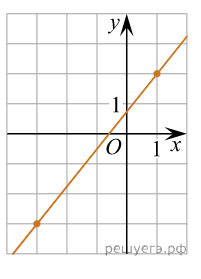
\includegraphics[align=t, width=1.2\linewidth]{../../../../exercises/lists/pics/G102M8cons2-4}
		\end{minipage}
	\item 
		\begin{minipage}[t]{\bodywidth}
			На рисунке изображён график функции вида \( f(x)=ax^{2}+bx+c \), где числа \( a \), \( b \) и \( c \)  — целые. Найдите значение \( f(3) \).
		\end{minipage}
		\hspace{0.02\linewidth}
		\begin{minipage}[t]{\picwidth}
			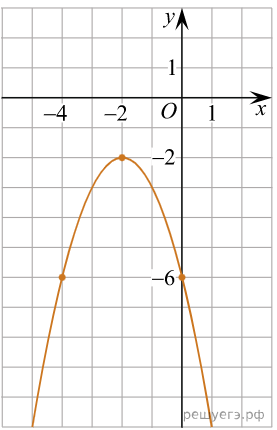
\includegraphics[align=t, width=1.2\linewidth]{../../../../exercises/lists/pics/G102M8cons2-1}
		\end{minipage}
	\item 
		\begin{minipage}[t]{\bodywidth}
			На рисунке изображён график функции \( f (x)=k\sqrt{x} \). Найдите \( f(2,56) \).
		\end{minipage}
		\hspace{0.02\linewidth}
		\begin{minipage}[t]{\picwidth}
			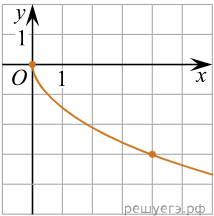
\includegraphics[align=t, width=1.2\linewidth]{../../../../exercises/lists/pics/G102M8cons2-2}
		\end{minipage}
	\item 
		\begin{minipage}[t]{\bodywidth}
			На рисунке изображён график функции вида \( f(x)=  \dfrac{k}{x+a} \).  Найдите значение x, при котором \( f (x) =0,15 \).
		\end{minipage}
		\hspace{0.02\linewidth}
		\begin{minipage}[t]{\picwidth}
			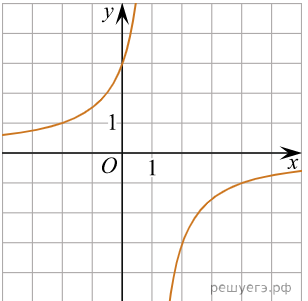
\includegraphics[align=t, width=1.3\linewidth]{../../../../exercises/lists/pics/G102M8cons2-3}
		\end{minipage}

	\item 
		\begin{minipage}[t]{\bodywidth}
			На рисунке изображён график функции вида \( f(x)=ax^{2}+bx+c \). Найдите значение \( f(8) \).
		\end{minipage}
		\hspace{0.02\linewidth}
		\begin{minipage}[t]{\picwidth}
			% TODO: \usepackage{graphicx} required
			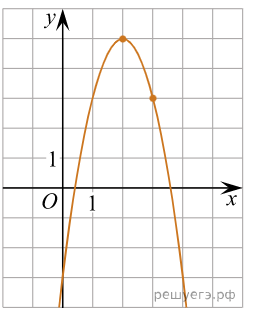
\includegraphics[align=t, width=1.2\linewidth]{../../../../exercises/lists/pics/G102M8cons2-5}
		\end{minipage}
	\item 
		\begin{minipage}[t]{\bodywidth}
			На рисунке изображён график функции \( f (x) =\dfrac{k}{x}+a \). Найдите, при каком значении \( x \) значение функции равно 0,8.
		\end{minipage}
		\hspace{0.02\linewidth}
		\begin{minipage}[t]{\picwidth}
			% TODO: \usepackage{graphicx} required
			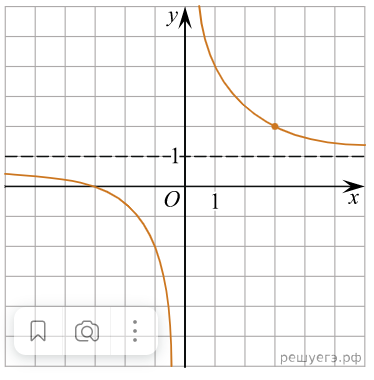
\includegraphics[align=t, width=1.3\linewidth]{../../../../exercises/lists/pics/G102M8cons2-6}
		\end{minipage}
	\item 
		\begin{minipage}[t]{\bodywidth}
			На рисунке изображён график функции \( f(x) =a^{x}+b \). Найдите значение \( x \), при котором \( f(x)=29 \).
		\end{minipage}
		\hspace{0.02\linewidth}
		\begin{minipage}[t]{\picwidth}
			% TODO: \usepackage{graphicx} required
			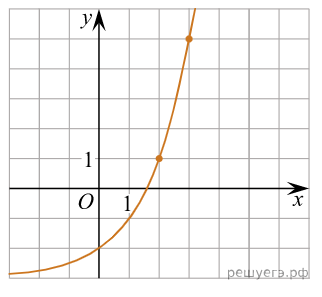
\includegraphics[align=t, width=1.3\linewidth]{../../../../exercises/lists/pics/G102M8cons2-7}
		\end{minipage}
		
		
	\end{listofex}
\end{consultation}
%END_FOLD

